\documentclass{beamer}

% Theme choice
\usetheme{Madrid}

% Optional packages
\usepackage{graphicx} % For including images
\usepackage{amsmath}  % For math symbols and formulas
\usepackage{hyperref} % For hyperlinks
\usepackage{listings}
\usepackage{xcolor}
\usepackage{tikz}
\usepackage[T1]{fontenc}

\lstdefinestyle{CStyle}{
  language=C,                    % Set the language to C
  basicstyle=\ttfamily\footnotesize\linespread{0.9}\tiny, % Set font style and size
  keywordstyle=\color{blue},      % Color of keywords
  commentstyle=\color{gray},      % Color of comments
  stringstyle=\color{red},        % Color of strings
  showstringspaces=false,         % Do not mark spaces in strings
  breaklines=true,                % Enable line breaks at appropriate places
  breakatwhitespace=false,        % Break lines at any character, not just whitespace
  numbers=left,                   % Show line numbers on the left
  numberstyle=\tiny\color{gray},  % Style for line numbers
  tabsize=4,                      % Set tab width
  keepspaces=true,                % Keep indentation spaces
  frame=single,                   % Add a border around the code
  aboveskip=0pt,                  % Reduce space above the code block
  belowskip=0pt,                   % Reduce space below the code block
  xleftmargin=7.5pt,                      % Add left padding (approx. 2.8mm or 10px)
  xrightmargin=15pt,                      % Add left padding (approx. 2.8mm or 10px)
}

% Title, author, date, and institute (optional)
\title[Parallel Programming. Repository structure]{Parallel Programming course. Repository structure}
\author{Obolenskiy Arseniy, Nesterov Alexander}
\institute{Nizhny Novgorod State University}

\date{\today} % or \date{Month Day, Year}

% Redefine the footline to display both the short title and the university name
\setbeamertemplate{footline}{
  \leavevmode%
  \hbox{%
    \begin{beamercolorbox}[wd=.45\paperwidth,ht=2.5ex,dp=1ex,leftskip=1em,center]{author in head/foot}%
        \usebeamerfont{author in head/foot}\insertshortinstitute % Displays the university name
    \end{beamercolorbox}%
    \begin{beamercolorbox}[wd=.45\paperwidth,ht=2.5ex,dp=1ex,leftskip=1em,center]{author in head/foot}%
      \usebeamerfont{author in head/foot}\insertshorttitle % Displays the short title
    \end{beamercolorbox}%
    \begin{beamercolorbox}[wd=.1\paperwidth,ht=2.5ex,dp=1ex,rightskip=1em,center]{author in head/foot}%
      \usebeamerfont{author in head/foot}\insertframenumber{} / \inserttotalframenumber
    \end{beamercolorbox}}%
  \vskip0pt%
}

\begin{document}

\begin{frame}
    \titlepage
\end{frame}

\begin{frame}{Contents}
    \tableofcontents
\end{frame}

\section{The introduction to the repository}

\begin{frame}[fragile]{Parallel programming technologies}
  \begin{itemize}
    \item \textbf{MPI}
    \item OpenMP
    \item TBB
    \item std::thread
  \end{itemize}
\end{frame}

\begin{frame}[fragile]{Step-by-step guide to build the project}
  \begin{itemize}
    \item Download all submodules
    \item Set up your environment
    \item Build the project with CMake
  \end{itemize}
\end{frame}

\begin{frame}[fragile]{Download all submodules \& Set up your environment}

  \lstset{style=CStyle, caption=Git submodules}
  \begin{lstlisting}
    git submodule update --init --recursive
  \end{lstlisting}

    \lstset{style=CStyle, caption=Download MPI}
  \begin{lstlisting}
    // Windows
    msmpisdk.msi & msmpisetup.exe
    // Linux (gcc and clang)
    sudo apt install -y mpich openmpi-bin libopenmpi-dev
    // MacOS (apple clang)
    brew install open-mpi
  \end{lstlisting}

\end{frame}

\begin{frame}[fragile]{Build the project with help CMake}

  \lstset{style=CStyle, caption=Configure the build}
  \begin{lstlisting}
    cmake -S <source code/path to CMakeLists.txt> \
          -B <build directory> \
          -D USE_SEQ=ON \
          -D USE_MPI=ON \ 
          -D USE_FUNC_TESTS=ON \
          -D USE_PERF_TESTS=ON \
          -D CMAKE_BUILD_TYPE=Release ..
  \end{lstlisting}

  \lstset{style=CStyle, caption=Build the project}
  \begin{lstlisting}
    cmake --build <build directory> \
          --config Release \
          --parallel
  \end{lstlisting}

\end{frame}

\section{How to submit your work}

\begin{frame}[fragile]{Directories}
  \begin{table}[h!]
    \resizebox{8cm}{!} {
      \begin{tabular}{| p{4.2 cm} | p{4.2 cm} |}
      \hline
      \textbf{Directory} & \textbf{What is it?} \\
      \hline
      \textbf{.github/workflows} & CI \\
      \hline
      \textbf{1stsamples} & Simple examples \\
      \hline
      \textbf{3rdparty} & Auxiliary libraries \\
      \hline
      \textbf{cmake} & CMake scripts \\
      \hline
      \textbf{modules} & API source code \\
      \hline
      \textbf{scripts} & Auxiliary scripts \\
      \hline
      \textbf{tasks} & Students tasks \\
      \hline
    \end{tabular}
    }
    \caption{Root directories}
  \end{table}

  \begin{table}[h!]
    \resizebox{8cm}{!} {
    \begin{tabular}{| p{4.2 cm} | p{4.2 cm} |}
      \hline
      \textbf{Directory} & \textbf{What is it?} \\
      \hline
      \textbf{mpi} & MPI \\
      \hline
      \textbf{omp} & OpenMP \\
      \hline
      \textbf{seq} & Sequential \\
      \hline
      \textbf{stl} & std:thread \\
      \hline
      \textbf{tbb} & Threading Building Blocks \\
      \hline
    \end{tabular}
    }
    \caption{Tasks directories}
  \end{table}

\end{frame}

\begin{frame}[fragile]{Directories}
  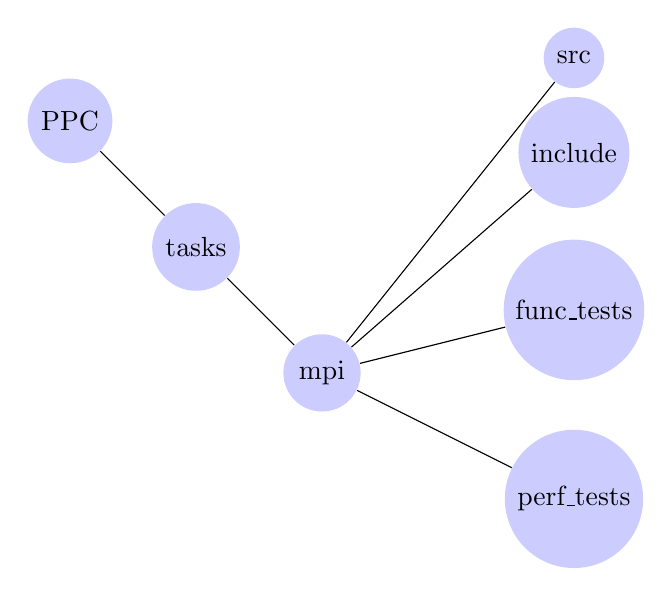
\begin{tikzpicture}
  [scale=.8,auto=left,every node/.style={circle,fill=blue!20}]
  \node (n1) at (1,10) {PPC};
  \node (n2) at (3,8)  {tasks};
  \node (n3) at (5,6)  {mpi};
  \node (n4) at (9,11)  {src};
  \node (n5) at (9,9.5) {include};
  \node (n6) at (9,7) {func\_tests};
  \node (n7) at (9,4) {perf\_tests};

  \foreach \from/\to in {n1/n2,n2/n3,n3/n4,n3/n5,n3/n6,n3/n7}
    \draw (\from) -- (\to);

\end{tikzpicture}
\end{frame}

\section{API of the course's repository}

\begin{frame}[fragile]{Task's prototype}
  \lstset{style=CStyle, caption=include/ops\_seq.hpp}
  \begin{lstlisting}
    class TestTaskSequential : public ppc::core::Task {
     public:
      explicit TestTaskSequential(std::shared_ptr<ppc::core::TaskData> taskData_) : Task(std::move(taskData_)) {}
      bool pre_processing() override;
      bool validation() override;
      bool run() override;
      bool post_processing() override;
    
     private:
      int input_{}, res{};
    };
  \end{lstlisting}
\end{frame}

\begin{frame}[fragile]{Task's source code}
  \lstset{style=CStyle, caption=src/ops\_seq.cpp | pre\_processing}
  \begin{lstlisting}
    bool nesterov_a_test_task_seq::TestTaskSequential::pre_processing() {
      internal_order_test();
      // Init value for input and output
      input_ = reinterpret_cast<int*>(taskData->inputs[0])[0];
      res = 0;
      return true;
    }
  \end{lstlisting}

  \lstset{style=CStyle, caption=src/ops\_seq.cpp | validation}
  \begin{lstlisting}
    bool nesterov_a_test_task_seq::TestTaskSequential::validation() {
      internal_order_test();
      // Check count elements of output
      return taskData->inputs_count[0] == 1 && taskData->outputs_count[0] == 1;
    }
  \end{lstlisting}
\end{frame}

\begin{frame}[fragile]{Task's source code}
  \lstset{style=CStyle, caption=src/ops\_seq.cpp | run}
  \begin{lstlisting}
    bool nesterov_a_test_task_seq::TestTaskSequential::run() {
      internal_order_test();
      for (int i = 0; i < input_; i++) {
        res++;
      }
      return true;
    }
  \end{lstlisting}

  \lstset{style=CStyle, caption=src/ops\_seq.cpp | post\_processing}
  \begin{lstlisting}
    bool nesterov_a_test_task_seq::TestTaskSequential::post_processing() {
      internal_order_test();
      reinterpret_cast<int*>(taskData->outputs[0])[0] = res;
      return true;
    }
  \end{lstlisting}
\end{frame}

\begin{frame}[fragile]{Task's functional tests}
  \lstset{style=CStyle, caption=func\_tests/main.cpp}
  \begin{lstlisting}
    TEST(Sequential, Test_Sum_10) {
      const int count = 10;
    
      // Create data
      std::vector<int> in(1, count);
      std::vector<int> out(1, 0);
    
      // Create TaskData
      std::shared_ptr<ppc::core::TaskData> taskDataSeq = std::make_shared<ppc::core::TaskData>();
      taskDataSeq->inputs.emplace_back(reinterpret_cast<uint8_t *>(in.data()));
      taskDataSeq->inputs_count.emplace_back(in.size());
      taskDataSeq->outputs.emplace_back(reinterpret_cast<uint8_t *>(out.data()));
      taskDataSeq->outputs_count.emplace_back(out.size());
    
      // Create Task
      nesterov_a_test_task_seq::TestTaskSequential testTaskSequential(taskDataSeq);
      ASSERT_EQ(testTaskSequential.validation(), true);
      testTaskSequential.pre_processing();
      testTaskSequential.run();
      testTaskSequential.post_processing();
      ASSERT_EQ(count, out[0]);
    }    
  \end{lstlisting}
\end{frame}

\begin{frame}[fragile]{TaskData structure}
  \lstset{style=CStyle, caption=TaskData}
  \begin{lstlisting}
    struct TaskData {
      std::vector<uint8_t *> inputs;
      std::vector<std::uint32_t> inputs_count;
      std::vector<uint8_t *> outputs;
      std::vector<std::uint32_t> outputs_count;
      enum StateOfTesting { FUNC, PERF } state_of_testing;
    };
  \end{lstlisting}
  \lstset{style=CStyle, caption=Functions order}
  \begin{lstlisting}
    std::vector<std::string> right_functions_order  = 
        {"validation", 
         "pre_processing", 
         "run", 
         "post_processing"};
  \end{lstlisting}
\end{frame}

\begin{frame}[fragile]{Task's performance tests - part 1}
  \lstset{style=CStyle, caption=perf\_tests/main.cpp}
  \begin{lstlisting}
    TEST(sequential_example_perf_test, test_pipeline_run) {
      const int count = 100;
    
      // Create data
      std::vector<int> in(1, count);
      std::vector<int> out(1, 0);
    
      // Create TaskData
      std::shared_ptr<ppc::core::TaskData> taskDataSeq = std::make_shared<ppc::core::TaskData>();
      taskDataSeq->inputs.emplace_back(reinterpret_cast<uint8_t *>(in.data()));
      taskDataSeq->inputs_count.emplace_back(in.size());
      taskDataSeq->outputs.emplace_back(reinterpret_cast<uint8_t *>(out.data()));
      taskDataSeq->outputs_count.emplace_back(out.size());
    
      // Create Task
      auto testTaskSequential = std::make_shared<nesterov_a_test_task_seq::TestTaskSequential>(taskDataSeq);
  \end{lstlisting}
\end{frame}

\begin{frame}[fragile]{Task's performance tests - part 2}
  \lstset{style=CStyle, caption=perf\_tests/main.cpp}
  \begin{lstlisting}
      // Create Perf attributes
      auto perfAttr = std::make_shared<ppc::core::PerfAttr>();
      perfAttr->num_running = 10;
      const auto t0 = std::chrono::high_resolution_clock::now();
      perfAttr->current_timer = [&] {
        auto current_time_point = std::chrono::high_resolution_clock::now();
        auto duration = std::chrono::duration_cast<std::chrono::nanoseconds>(current_time_point - t0).count();
        return static_cast<double>(duration) * 1e-9;
      };
    
      // Create and init perf results
      auto perfResults = std::make_shared<ppc::core::PerfResults>();
    
      // Create Perf analyzer
      auto perfAnalyzer = std::make_shared<ppc::core::Perf>(testTaskSequential);
      perfAnalyzer->pipeline_run(perfAttr, perfResults);
      ppc::core::Perf::print_perf_statistic(perfResults);
      ASSERT_EQ(count, out[0]);
    }
  \end{lstlisting}
\end{frame}

\begin{frame}[fragile]{Practice}
  Practice
\end{frame}

\begin{frame}{References}
  \begin{itemize}
    \item PPC Repository \href{https://github.com/learning-process/parallel\_programming\_course}{https://github.com/learning-process/parallel\_programming\_course}
  \end{itemize}
\end{frame}

\end{document}
